\chapter{Preâmbulo matemático}
\section{Produto escalar e produto vetorial de vetores}
Dados dois vetores, define-se o seu \emph{produto escalar} (ou \emph{produto
interno}) como o escalar que se obtém multiplicando os módulos dos dois vetores
e o cosseno do ângulo entre eles. Assim, se $\vec a$ e $\vec b$ forem os dois
vetores e $\theta$ for o ângulo que definem, o produto escalar
é\footnote{Nestes apontamentos usa-se uma convenção tipográfica usual em física,
  em que se representa o módulo de um vetor $\vec a$ por $a$: a mesma letra, mas
sem a setinha por cima.}
\begin{equation}
  \vec a\cdot\vec b= ab\cos\theta.
\end{equation}
É imediato verificar que o produto escalar de dois vetores pode ser positivo (se
o ângulo entre eles for menor que 90\deg), negativo (se for maior que 90\deg) ou
nulo (se os dois vetores forem perpendiculares). Verifica-se também
que este produto é comutativo, isto é, $\vec a\cdot\vec b=\vec b\cdot\vec a$.


Sejam respetivamente $(a_x,\,a_y,\,a_z)$ e $(b_x,\,b_y,\,b_z)$ as componentes
dos vetores $\vec a$ e $\vec b$ relativamente a alguma base ortonormada
pré-escolhida, formada por versores (vetores com norma 1) $\he_x$, $\he_y$ e
$\he_z$. Isto quer dizer que estes dois vetores se podem escrever como as
combinações lineares dos vetores da base seguintes
\begin{align*}
  \vec a&=a_x\he_x+a_y\he_y+a_z\he_z&
  \vec b&=b_x\he_x+b_y\he_y+b_z\he_z.
\end{align*}
O produto escalar destes dois vetores pode então desenvolver-se como
\begin{align*}
  \vec a\cdot\vec b&=
  (a_x\he_x+a_y\he_y+a_z\he_z) \cdot (b_x\he_x+b_y\he_y+b_z\he_z)\\
  &=a_xb_x(\he_x\cdot\he_x)+ a_xb_y(\he_x\cdot\he_y)+ a_xb_z(\he_x\cdot\he_z)\\
  &+a_yb_x(\he_y\cdot\he_x)+ a_yb_y(\he_y\cdot\he_y)+ a_yb_z(\he_y\cdot\he_z)\\
  &+a_zb_x(\he_z\cdot\he_x)+ a_zb_y(\he_z\cdot\he_y)+ a_zb_z(\he_z\cdot\he_z)
\end{align*}
Mas os produtos escalares de versores da base diferentes são nulos (porque eles
são todos perpendicuares entre si) e os produtos escalares de um qualquer versor
da base consigo próprio é 1 (porque o módulo dos versores é 1 e o cosseno do
ângulo [nulo] que um vetor faz consigo próprio também é 1), isto é,
\begin{align*}
  \he_x\cdot\he_x=\he_y\cdot\he_y=\he_z\cdot\he_z=1\\
  \he_x\cdot\he_y=\he_y\cdot\he_z=\he_z\cdot\he_x=0.
\end{align*}
Substituindo em cima, obtemos uma forma alternativa para o produto escalar de
dois vetores:
\begin{equation}
  \vec a\cdot\vec b=a_xb_x+a_yb_y+a_zb_z.
\end{equation}

Define-se também o \emph{produto vetorial} ou \emph{produto externo} de vetores.
Como o próprio nome indica, o produto vetorial de dois vetores é ainda um
vetor.%\footnote{Ao contrário do produto escalar de vetores que, como acabámos de
%ver, é... Um escalar.}.
A norma do produto escalar de dois vetores é o produto
das suas normas e do seno do ângulo entre eles:
\begin{equation}
  \|\vec a\times\vec b\|=ab\sin\theta;
\end{equation}
a sua direção é a perpendicular ao plano definido pelos dois vetores que se
multiplicam e o sentido é o definido pela regra da mão direita\footnote{%
  \parbox[t]{0.8\textwidth}{Há várias formas de enunciar esta regra, pode
    encontrá-las todas rapidamente numa pesquisa na web (experimente usar
    ``cross product right hand rule'' como expressão de busca). Escolha a que
    preferir. Eu gosto desta: oriente o indicador da mão direita como o primeiro
    vetor no produto e o médio da mesma mão como o segundo; o polegar indica
  então o sentido do produto vetorial (veja a figura ao lado, retirada da
  Wikipedia)}\hfill
  \parbox[t]{1.8cm}{%
    \raisebox{-0.8\height}{%
      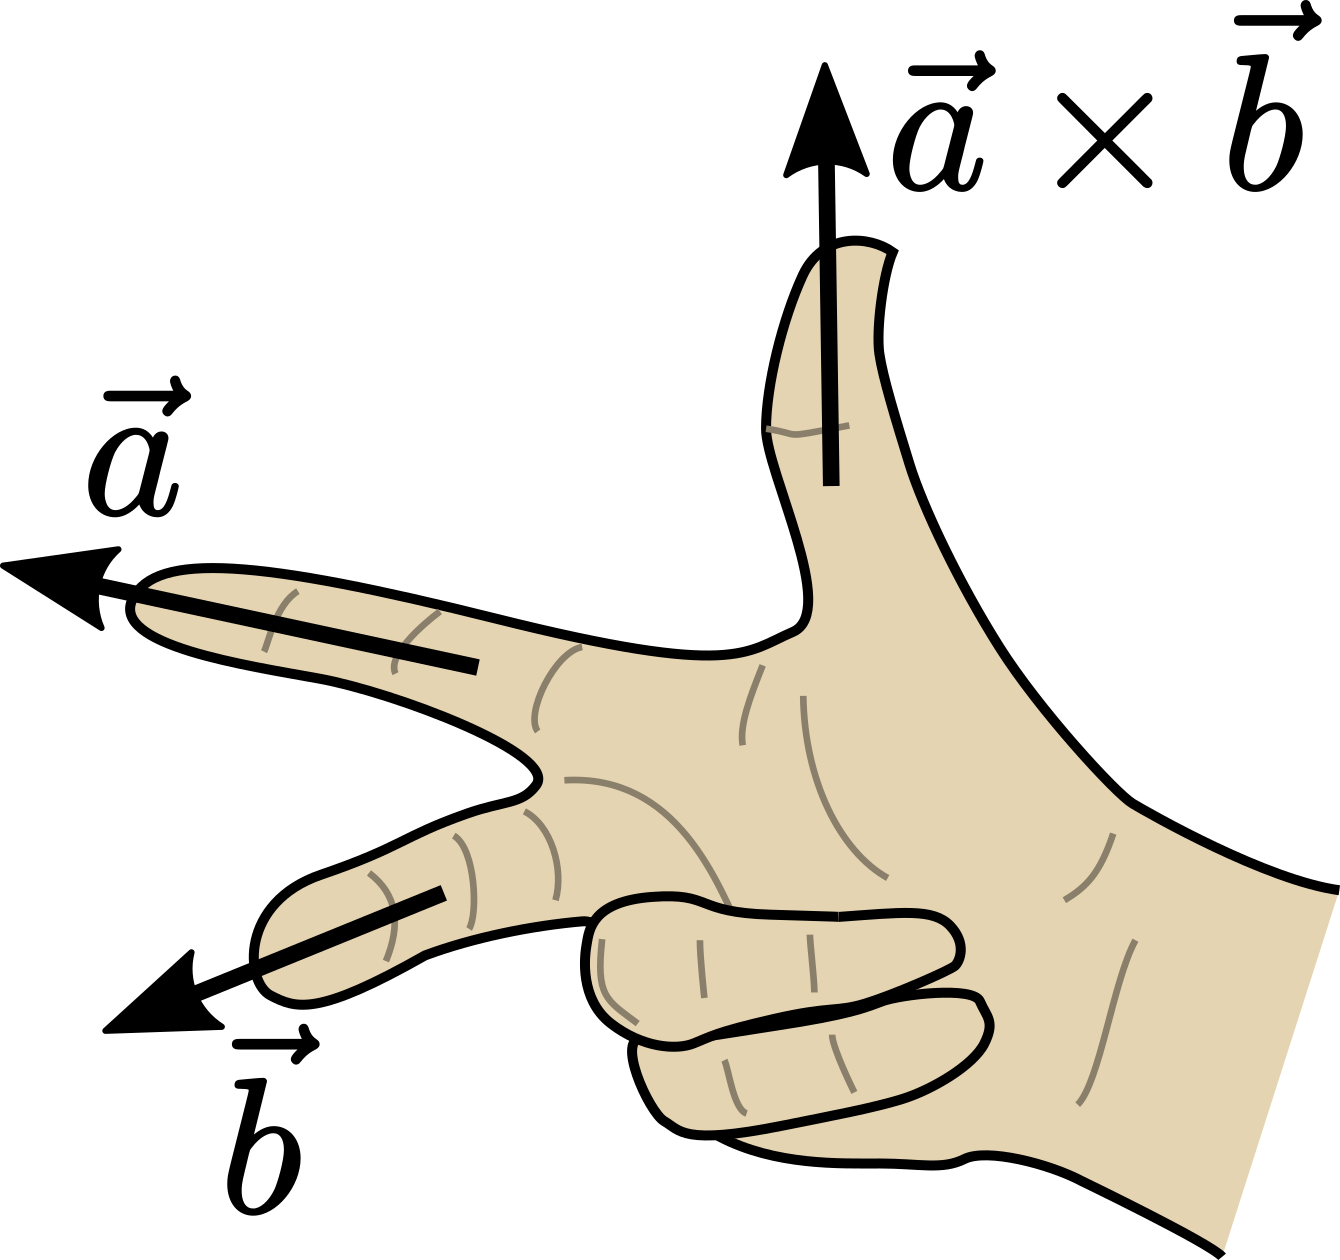
\includegraphics[width=1.7cm]{figs/f10-010.png}
    }
  }
}.
O produto vetorial assim definido é \emph{anticomutativo}, isto é, o sinal do
resultado é trocado se trocarmos a ordem dos fatores: $\vec a\times\vec b=-\vec
b\times\vec a$. Constata-se também que
\begin{align}
  \he_x\times\he_y&=\he_z&
  \he_y\times\he_z&=\he_x&
  \he_z\times\he_x&=\he_y.
\end{align}
Munidos destas igualdades (e das que resultam trocando a ordem dos fatores nos
seus lados esquerdos) obtemos uma expressão para o cálculo do vetor produto
vetorial em termos das componentes dos dois vetores multipicados externamente.
Sejam, como há pouco, $a_x,\,a_y,\,a_z$ e $b_x,\,b_y,\,b_z$ as componentes de
dois vetores $\vec a $ e $\vec b$ relativamente a uma base ortonormada formada
por vetores unitarios $\he_x$ $\he_y$, $\he_z$. Então,
\begin{equation*}
  \vec a = a_x\he_x+a_y\he_y+a_z\he_z\rule{2cm}{0mm}
  \vec b = b_x\he_x+b_y\he_y+b_z\he_z,
\end{equation*}
e, assim,
\begin{align*}
  \vec a \times \vec b &=
  (a_x\he_x+a_y\he_y+a_z\he_z)\times
  (b_x\he_x+b_y\he_y+b_z\he_z)\\
  &=
  (a_yb_z-a_zb_y)\he_x+(a_zb_x-a_xb_z)\he_y+(a_xb_y-a_yb_x)\he_z.
\end{align*}
Esta expressão para o produto vetorial de dois vetores em termos das componentes
dos vetores multiplicados é fácil de memorizar notando que pode também ser vista
como o determinante da matriz simbólica (verifique):
\begin{equation}
  \vec a\times\vec b =\det
  \begin{bmatrix}
    \he_x&\he_y&\he_z\\
    a_x&a_y&a_z\\
    b_x&b_y&b_z
  \end{bmatrix}.
\end{equation}

O produto vetorial não é comutativo (é anticomutativo, como vimos) e também não
é associativo. O produto vetorial de três vetores satisfaz as igualdades
\begin{equation}\label{eq:tcp}
\begin{split}
\vec a\times(\vec b\times\vec c)&=\vec b(\vec a\cdot\vec c)-(\vec a\cdot\vec
b)\vec c\\
(\vec a\times\vec b)\times\vec c&=\vec b(\vec a\cdot\vec c)-\vec a(\vec
b\cdot\vec c)
\end{split}
\end{equation}

\subsection{Áreas de paralelogramos e volumes de paralelipípedos}
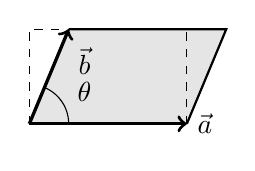
\begin{tikzpicture}[baseline=(current bounding box.north)]
%\small
\coordinate(O) at (0,0);
\coordinate(a) at (2,0);
\coordinate(b) at (0.5,1.2);
\coordinate(ab) at (2.5,1.2);
\fill [gray!20] (O) -- (a) -- (ab) -- (b) --cycle;
\draw [very thick, ->] (O) --(a) node[right]{$\vec a$};
\draw [very thick, ->] (O) --(b) node[shift={(2mm,-4mm)}]{$\vec b$};
\draw [thick] (a) -- (ab) -- (b);
\draw [dashed] (O) -- (O|-b) --(b);
\draw [dashed] (a) -- (a|-b);
\begin{scope}
\clip (b)--(O) --(a);
\draw (O) circle (0.5cm) node[shift={(7mm,4mm)}] {$\theta$};
\end{scope}
\end{tikzpicture}
\hfill
\begin{minipage}[t]{0.8\textwidth}
Consideremos a área do paralelogramo formado por dois vetores $\vec a$ e $\vec
b$ (ver a figura ao lado). Seja $\theta$ o ângulo entre os dois vetores.
Claramente, aquela área é igual à do retângulo com base $a=\|\vec a\|$ e altura
$b\sin\theta$, igual à do paralelogramo inicial. A área considerada é pois
\end{minipage}
\begin{equation}
A=ab\sin\theta=\|\vec a\times\vec b\|.
\end{equation}

Consideremos agora um terceiro vetor $\vec c$, não coplanar com $\vec a$ e $\vec
b$. Seja $\phi$ o ângulo entre $\vec c$ e a normal ao plano definido pelos
vetores $\vec a$ e $\vec b$. Com um argumento semelhante ao que acabámos de
usar para calcular a área de um paralelogramo, prova-se que o volume deste
paralelipípedo é
\begin{equation}
V=b\cos\phi A = c \|\vec a\times\vec b\| \cos\phi=
\left|\vec c\cdot\vec a\times\vec b\right|.
\end{equation}

\section{Operadores diferenciais}
As equações de Maxwell são quatro equações às derivadas parciais dos campos
elétrico e magnético que traduzem localmente\footnote{Isto é, como igualdades
que relacionam o valor de funções em cada ponto do espaço.} as leis integrais
do eletromagnetismo que foram estudadas na cadeira de Física Geral II, a saber:
a lei de Gauss do campo elétrico (e uma que desempenha um papel semelhante para
o campo magnético), a lei de Faraday e a lei de Ampère. Estas equações envolvem
os operadores diferenciais divergência e rotacional, que vamos agora,
rapidamente, recordar.

\section*{Divergência de um campo vetorial}
A divergência de um campo vetorial é um escalar igual ao fluxo do campo atrvés
de uma superfície fechada por unidade de volume.  De um modo talvez mais
intuitivo (mas muito menos preciso), podemos dizer que é a \emph{``quantidade''
de campo que ``sai''} desse ponto por unidade de volume. A
Figura~\ref{fig:10-020} ilustra este significado intuitivo da divergência de um
campo vetorial.
\begin{figure}[htb]
  {\centering
    \begin{tikzpicture}
	\small
	\coordinate(P) at (-2,0);
	\coordinate(Q) at (2,0);
	\foreach \q in {0,30, 60, 90, 120,150,180,210,240,270,300,330} {
		\draw [->-] (P) -- +(\q:1cm);
		\draw [-<-] (Q) -- +(\q:1cm);
	};
	\node at (P) [shift={(3mm,-3mm)}, fill=white,inner sep=2pt]{$P$};
	\node at (Q) [shift={(3mm,-3mm)}, fill=white,inner sep=2pt]{$Q$};
\end{tikzpicture}
\par
  }
  \caption{À esquerda, exemplo de um campo com divergência positiva no ponto
  $P$; à direita o campo tem divergência negativa no ponto
  $Q$.\label{fig:10-020}}
\end{figure}


Pode demonstrar-se (mas não o faremos aqui) que, usando coordenadas cartesianas,
a divergência de um campo vetorial $\vec V$ é dada por
\begin{equation}\label{eq:divcart}
  \div\vec V=\pd{V_x}{x} + \pd{V_y}{y}+\pd{V_z}{z}.
\end{equation}
Introduzindo agora o símbolo vetorial ``nabla'' 
\begin{equation*}
  \vec \nabla = (\pd{}{x},\, \pd{}{y},\, \pd{}{z}),
\end{equation*}
a divergência de $\vec V$ pode ainda escrever-se de forma mais condensada como
o produto escalar de nabla e $\vec V$:
\begin{equation}
  \div\vec V=\vec\nabla\cdot\vec V.
\end{equation}

Em coodenadas polares cilíndricas $(r,\,\varphi,\,z)$, a divergência de um campo
vetorial $\vec V=V_r\he_r+V_\varphi\he_\varphi+V_z\he_z$ tem a forma
\begin{equation}
\div\vec V=\frac{1}{r}\pd{(rV_r)}{r}+\pd{V_\varphi}{\varphi}+\pd{A_z}{z}
\end{equation}
e, em coordenadas polares esféricas $(r,\,\theta,\,\varphi)$, 
\begin{equation}
\div \vec A=\frac{1}{r^2}\pd{(r^2A_r)}{r}+
    \frac{1}{r\sin\theta}\pd{}{\theta}(A_\theta\sin\theta)+
    \frac{1}{r\sin\theta}\pd{A_\varphi}{\theta}
\end{equation}

\section*{Rotacional de um campo vetorial}
O rotacional de um campo vetorial é um vetor igual à circulação do campo por
unidade de área. A sua direção é a perpendicular ao plano onde a circulação tem
o valor máximo. Em termos intuitivos (mas terivelmente imprecisos), o rotacional
dá uma ideia de \emph{``quanto'' é que o campo ``roda''} num ponto; a sua
direção é do ``eixo'' dessa ``rotação'' e o sentido é o dado pela regra da mão
direita a partir do sentido da ``rotação'' do campo. 

O rotacional de um campo $\vec V$ é, em coordenadas cartesianas, dado por
\begin{equation}\label{eq:rotcart}
  \rot\vec V=
  \left(\pd{V_z}{y}-\pd{V_y}{z},\; \pd{V_x}{z}-\pd{V_z}{x},\;
  \pd{V_y}{x}-\pd{V_x}{y}\right).
\end{equation}
Em termos do símbolo vetorial nabla, fica, mais sucintamente,
\begin{equation}
  \rot\vec V=\vec\nabla\times\vec V.
\end{equation}

Usando a primeira das igualdades da eq.~\eqref{eq:tcp}, encontramos uma
expressão para o rotacional do rotacional de um campo vetorial, que será útil
quando estuidarmos as ondas eletromagnéticas:
\begin{align}
\rot\rot \vec A&=\vec\nabla\times\vec\nabla\times\vec V=
\vec \nabla(\vec\nabla\cdot\vec V)-\nabla^2\vec V\nonumber\\
&=\grad\div \vec V-\lap\vec V,
\end{align}
onde $\lap\vec A$ representa o \emph{laplaciano} do campo vetorial$\vec V$, um
operador diferencial de segunda ordem, igual à soma das duplas derivadas não
cruzadas do campo,
\begin{equation}
\lap X =
\pdd{F}{x}+
\pdd{F}{y}+
\pdd{F}{z},\qquad\text{para qualquer função escalar ou vetorial $F$}
\end{equation}
{\small%
  Feita esta abreviadíssima explicação sobre os operadores $\div$ e $\rot$,
  talvez não seja pior referir alguns factos mais básicos da ``vida secreta
  das derivadas''. Uma função crescente tem uma variação positiva quando a
  variável de que depende sofre um acréscimo; logo, a sua taxa de variação
  (variação da função a dividir pelo acréscimo da variável) é positiva, logo a
  sua derivada (outro nome para a taxa de variação) é positiva. Do mesmo modo,
  uma função decrescente tem derivada negativa. Uma função constante não é
  crescente nem decrescente; logo, não tem derivada positiva nem negativa, tem
  derivada nula.  Uma função que atinge um valor extremo (máximo ou mínimo) para
  um dado valor da variável de que depende, nesse ponto não é crescente nem
  decrescente: tem derivada nula nesse ponto.

  Quando estudamos funções de várias variáveis (como é o caso agora), estas
  regras ainda se aplicam mas têm que ser consideradas com cuidado porque a
  função pode ser crescente relativamente aos acréscimos de uma variável,
  decrescente com acréscimos de outra variável e constante com acréscimos de uma
  terceira variável. Assim, uma função que depende da posição e do tempo e que
  num dado ponto tem um valor que vai paulatinamente aumentando à medida que o
  tempo passa, é uma função que tem, nesse ponto, derivada temporal positiva. Se
  o seu valor num dado ponto se mantém inalterado com a passagem do tempo, então
  a sua derivada temporal, nesse ponto, é nula. E etc, etc, etc, acho que destes
  dois exemplos já se vai percebendo a lógica geral.

  A derivada de uma função de várias variáveis em ordem a uma delas é ainda, em
  geral, uma função dessas mesmas variáveis. Como tal, pode fazer sentido
  derivá-la novamente, em ordem à mesma variável ou em ordem a outra qualquer. O
  teorema de Swartz garante que esta derivada não depende da ordem com que se
  fazem cada uma das derivações:
  \begin{equation*}
    \cpdd{f}{x}{y}=
    \cpdd{f}{y}{x},\qquad\text{qualquer que seja a função $f$}
  \end{equation*}
}

